\documentclass{article}
\usepackage[utf8]{inputenc}
\usepackage[T1]{fontenc}
\usepackage{amsmath}
\usepackage{amssymb}
\usepackage{proof}
\usepackage{soul}
\usepackage{xcolor}
\usepackage{enumerate}
\usepackage{hyperref}
\usepackage{listings}
\usepackage{graphicx}
\usepackage{lmodern}
\usepackage{float}
\usepackage{todonotes}
\usepackage{subfigure}
\usepackage{booktabs}
\usepackage{rotating}
\usepackage[binary-units]{siunitx}
\usepackage[backend=biber]{biblatex}

\addbibresource{sources.bib}
\title{Linearizable Wait-Free Queue \\ \large Project 13 -- Report \\ \vspace{1em} \small ($184.726$) Advanced Multiprocessor Programming\\Technical University of Vienna}
\author{Philipp Daniel Birkl (01326660) \and Hannes Brantner (01614466)}

\date{Summer Semester 2020}

\DeclareSIUnit\mops{MOPS}

\newcommand{\GLQ}{\texttt{GLQ}}
\newcommand{\LFQ}{\texttt{LFQ}}
\newcommand{\WFQ}{\texttt{WFQ}}

\begin{document}
\maketitle{}
\section{Theory}
\subsection{Overview}
The main task in this project was to implement and benchmark the concurrent wait-free non-blocking FIFO queue for an asynchronous shared memory system proposed by \cite{WFQ}. Non-blocking data structures are favorable because they do not suffer from deadlock for example. The wait-free and lock-free progress guarantee entail a non-blocking data structure. A wait-free progress guarantee means that every thread can perform an arbitrary operation on the corresponding data structure object within a finite number of steps. Therefore, tight bounds can be given for any operation in real-time multiprocessor systems. Wait-free data structures in the past had the problem that they performed worse than lock-free data structures in terms of latency and throughput because they provided a better progress guarantee. A lock-free progress guarantee means that some thread can perform an arbitrary operation on the corresponding data structure object within a finite number of steps. The proposed wait-free queue tries to coordinate threads over \texttt{fetch-and-add} primitives when contention is not too high, otherwise it uses also \texttt{compare-and-swap} primitives. As \texttt{fetch-and-add} primitives are guaranteed to succeed, this approach should be very performant. If the contention is higher, the threads are also coordinated over \texttt{compare-and-swap} primitives, which are not guaranteed to succeed, because the comparison value could be different to the actual value. Memory is reclaimed using an epoch based reclamation scheme and hazard pointers. The proposed wait-free queue also ensures that all data structure operations are linearizable. This means the operations take effect instantaneously sometime between invocation and retirement. The wait-free queue is implemented using the fast-path-slow-path methodology proposed in \cite{FPSP}. Each operation has a fast path and a slow path, where the fast path ensures performance and the slow path ensures wait-freedom. The threads executing a fast path help threads executing a slow path to complete their operation in a finite number of steps. In general a queue is not the best data structure to parallelize due to its intrinsic sequential behavior. 
\subsection{High-level design}
The pseudo code shown in \cite{WFQ} assumes a sequentially consistent memory model. As most modern architectures only support a total store order memory model where stores can be ordered after loads, memory fences must be added at crucial points to ensure the correctness of the implementation. The high-level structure of the fast-path operations of the wait-free queue is given in the following code listing of an obstruction-free queue, where $Q$ denotes the infinite array, $H$ denotes the unbounded head index and $T$ denotes the unbounded tail index. An obstruction-free progress guarantee means that a single thread can execute a data structure operation in a finite number of steps in isolation and every operation is non-blocking. Initially each cell of the infinite array contains the value $\bot$.
\begin{lstlisting}[mathescape, language=C, label=OFQ, caption=obstruction-free queue]
void enqueue(void *elem) {
    do t = FAA(&T,1)
    while (!CAS(&Q[t],$\bot$,x));
}

void *dequeue() {
    do h = FAA(&H,1)
    while (CAS(&Q[h],$\bot$,$\top$) && T > h);
    return (Q[h] == $\top$ ? EMPTY : Q[h]);
}
\end{lstlisting}
As this implementation would be susceptible to livelock and would not provide a wait-free progress guarantee, the iterations of both while loops must be bounded. If the operation has not succeeded within that bound, the corresponding slow path operation is called to ensure wait-freedom. The infinite array of the wait-free queue is emulated using a singly-linked list of equal-sized array segments called $nodes$, where the individual values are stored in $cells$ that have globally ascending indices. Each thread maintains a local pointer to the next $head$ node for dequeueing and a local pointer to the next $tail$ node for enqueuing. If a cell index does not exist in the emulated infinite array, a new node is allocated. Unused nodes are periodically reclaimed by a single thread scanning every thread's $head$ node, $tail$ node, and hazard pointers to determine these nodes.
\subsection{Wait-freedom}
Wait-freedom is achieved by turning contending threads that prevent another thread's operation to succeed into helpers such that all operations finish in a finite number of steps. An example that can be derived by looking at Listing \ref{OFQ}, an enqueue on the fast-path may never succeed because contending dequeues mark ever cell they visit as unusable by storing $\top$ into it. The local states of all threads called $handles$ are linked in a ring, such that every thread can access every other thread's state variables. Therefore, before a dequeue marks a cell as unusable it, it tries to take the value of a contending enqueuer operating on the same cell that is the dequeuer's enqueue peer if it has a pending enqueue request in its local state. When the peer's operation completes, the enqueue peer is updated the the next handle in the ring. Every time an enqueue fails, the contending dequeuer will help some enqueue request to complete. If all contending dequeuers become the enqueuer's helper, the enqueue is guaranteed to succeed. Similarly a fast-path dequeue may never succeed because slow-path dequeuers may take its value. Therefore, each thread needs to keep a pointer to the handle of a dequeue peer that is helped if it has a pending dequeue request in its local state when both dequeues are contending by searching together for a value to dequeue. A dequeue on the slow path will eventually succeed if all contending dequeues will help it to dequeue. When the peer's operation completes, the dequeue peer is updated the the next handle in the ring. This two methods are necessary to ensure wait-freedom for both queue operations.
\subsection{Structures of the wait-free queue}
The infinite array is emulated as a singly-linked list of nodes, which contain an array of cells. The nodes have ascending indices and also each cell has a unique globally ascending index. Each cell has also a pointer to an enqueue request or a dequeue request, but they may both be empty. The head cell index and the tail cell index are also stored in the struct of the queue. The thread local state contains the local head node and the local tail node pointers, a pointer to the next handle in the ring, the mentioned enqueue and dequeue requests, as well as pointers to the handles of the enqueue and the dequeue peer. It must also be mentioned that most of the pointers in the implementation provide two special values called $\top$ and $\bot$ to distinguish between an empty pointer that nobody has observed and an empty pointer that was already observed. For more detailed information about the used structures consult \cite{WFQ} or the appended commented source code of this project.
\subsection{Linearizable wait-free enqueue}
The fast-path enqueue is similarly to the obstruction-free queue presented in Listing \ref{OFQ} with the difference that the last acquired enqueue cell index is always saved and passed on to the slow-path enqueue, which is called if the patience is exhausted and the fast-path enqueue has not succeeded. The slow-path enqueue starts by the thread publishing its enqueue request in its handle. After that the enqueuer tries to complete the operation itself by also using \texttt{fetch-and-add} on the enqueue cell index and trying to deposit the value in the respective cell, which was claimed by also writing to the cell's enqueue request. This will stop when this operation succeeds or a contending dequeuer on the same cell helps the enqueuer and takes its value. The number of steps of each enqueue operation can be bounded by summing up the steps from the fast-path enqueue tries and the slow-path enqueue. As the loop iterations of the fast-path enqueue are at most \texttt{PATIENCE} iterations and the iterations of the first loop inside the slow-path enqueue are also bounded by $(n - 1)^2$ iterations where $n$ is the number of threads. Therefore, the overall number of steps can be bounded for every thread and there is a finite bound for the whole enqueue operation, which makes it wait-free. The linearization point for a fast-path enqueue is the timepoint where the thread has exchanged the value the corresponding cell using \texttt{compare-and-swap}. The linearization point for the slow-path enqueue is the last instruction of slow-path enqueue where the value is stored into the corresponding cell after eventually advancing the tail cell index. For more details about how the helper scheme works, wait-freedom and linearization points in detail consult \cite{WFQ} or the appended commented source code of this project. 
\subsection{Linearizable wait-free dequeue}
The fast-path dequeue is similarly to the obstruction-free queue presented in Listing \ref{OFQ} with the difference that the last acquired dequeue cell index is always saved and passed on to the slow-path dequeue, which is called if the patience is exhausted and the fast-path dequeue has not succeeded, and an eventual enqueue peer is helped at each visited cell. If a dequeuer succeeds, it mus help its dequeue peer before it returns the value. The slow-path dequeue starts by the thread publishing its dequeue request in its handle. Then the calling thread as well as other succeeding dequeuers call the dequeue helper method to complete the thread's operation in a finite number of steps. The number of steps of each dequeue operation can be bounded by summing up the steps from the fast-path dequeue tries and the slow-path dequeue. As the loop iterations of the fast-path dequeue are at most \texttt{PATIENCE} iterations and the iterations of the first loop inside the slow-path dequeue are also bounded by $(n - 1)^4$ iterations where $n$ is the number of threads. Therefore, the overall number of steps can be bounded for every thread and there is a finite bound for the whole dequeue operation, which makes it wait-free. The linearization points for dequeue operations are much more difficult to define than for the enqueue operation because there are lots of possibilities how a dequeue value can be acquired. Since also the helper methods for enqueuers and dequeuers play a big role here, the authors of \cite{WFQ} created a linearization procedure to correctly order linearization points of various concurrent queue operations. For more details about how the helper scheme works, wait-freedomness and linearization points in detail consult \cite{WFQ} or the appended commented source code of this project.
\subsection{Wait-free memory reclamation}
The wait-free queue implementation has only unused nodes that must be reclaimed. A node is no longer in use when both the head and tail cell indices have move past the cell indices present in the node and every enqueued value in the respective node has been dequeued. The queue struct is augmented with a pointer to the oldest node. To determine if every enqueued value in the respective node has been dequeued, the thread that is executing the cleanup method has access to all thread's local head and tail node pointers and it also uses the hazard pointers announced by each thread before doing an operation, which contain the node index they are working on. At every dequeue the cleanup method is called, which reclaims the memory used by unused nodes if there are enough unused nodes to reclaim. In this method also the head node and tail node indices of some threads will be updated if they point to nodes that are going to be deleted. This memory reclamation scheme is prone to thread failure. The cleanup method is also wait-free, since the amount of steps it takes to complete is finite, as all threads are visited and all unused segments are freed and both parameters are finite. Therefore, the dequeue operation is still wait-free after adding the cleanup call at every dequeue invocation. For more details about how the reclamation scheme works and wait-freedomness in detail consult \cite{WFQ} or the appended commented source code of this project.
\clearpage
\section{Evaluation}
\subsection{Introduction\label{sec:eval-intro}}
The goal of our evaluation was to analyze the performance metrics of the \WFQ~in comparison to two other queues that provided different progress guarantees to gain insight of their behavior in a real asynchronous shared memory system, as well as to try to falsify the correctness of the queue implementations. The following three queues were tested during the evaluation:
\begin{itemize}
    \item The \emph{global-lock queue} (\GLQ):\\It uses the ISO C++ standard library implementation \texttt{std::queue}, whose methods are accessed mutual exclusive. This is guaranteed by a \texttt{std::mutex} object that guards the enqueue and dequeue operation. Furthermore the pre-configured backing data-structure is used for \texttt{std::queue}, which defaults to the \texttt{std::dequeue} container.
    \item The \emph{lock-free queue} (\LFQ):\\It is presented by \citeauthor{LFQ} in his blog post \cite{LFQ}. This queue is built upon a set of \emph{SPMC} (single-producer multiple-consumer) queues and especially tuned for high throughput and low latency. For more details about the implementation refer to the blog post \cite{LFQEXPL} of \citeauthor{LFQEXPL}, which also explains the used theory behind the implementation.
    \item The \emph{wait-free queue} (\WFQ):\\It is presented by \citeauthor{WFQ} \cite{WFQ} in their paper and the implementation was discussed in the preceding section. It is an obstruction-free fetch-and-add queue that was augmented to provide wait-freedom. This obstruction-free base design is similar to the base algorithm used for LCRQ \cite{MA13}.
\end{itemize}

\paragraph{Evaluation overview}
In section \ref{sec:eval-methodology} the methodology is explained in detail, which should describe precisely how the performance metrics were collected and how the correctness of the three implementations was tried to falsify. The correctness test is described in \ref{sec:eval-methodology-correctness}, while \ref{sec:eval-methodology-benchmark} describes the benchmark test. In section \ref{sec:eval-benchmark} the performance metrics of each queue are discussed (sections \ref{sec:eval-benchmark-glq}-\GLQ, \ref{sec:eval-benchmark-lfq}-\LFQ, \ref{sec:eval-benchmark-wfq}-\WFQ). In section \ref{sec:eval-conlusion} all queues are compared and the impact of different design decisions and progress guarantees on various performance metrics is highlighted. Section \ref{sec:eval-results} contains all measured results in plots.
\clearpage
\subsection{Methodology\label{sec:eval-methodology}}
\paragraph{Programming language}
All the sources for this project were written in \texttt{C++} and compiled using the preliminary \texttt{C++20} standard. This programming language was chosen because it includes good libraries for threads as well as atomic operations, which are needed to build and test modern multi-threaded applications. Using the atomic library of \texttt{C++} for atomic instructions is much more convenient than using inline assembler. The implementation of the \WFQ{} queue\footnote{\WFQ{} implementation given by \citeauthor{WFQ}: \url{https://github.com/chaoran/fast-wait-free-queue}} written in the C programming language was completely rewritten in modern \texttt{C++} and thoroughly tested to ensure the correctness of our implementation. Another possible language would have been the \texttt{Java} programming language, but its garbage collector can easily invalidate wait-freedom claim made by the queue author and the language's support for atomic instructions is worse to the one provided by the \texttt{C++} standard. 
\paragraph{Supported queue data types} All three implemented queues only store pointers to objects, this was a necessity inherited by the implementation of the \WFQ, as it encodes state information as invalid pointers. To change that behavior, in depth modifications would have been necessary, potentially changing the intended workings of the queue by \citeauthor{WFQ}, leading to a potential performance difference. As memory can simply be allocated before the enqueue operation of the respective object, this does not limit the functionality of the queue, but it does limit the performance due to memory allocation and copying latency.
\paragraph{Evaluation software}
It was decided that all evaluations should be possible with one prebuilt executable, hindering the compiler in effectively optimizing the implementations of a fraction of queues based on constant pre-configured parameters, like unrolling loops or reordering instructions. This does help in providing a more real-life evaluation scenario as too aggressive compiler optimizations would be suppressed. To provide an overview about the extensive parametrization capabilities of our evaluation executable, a help command line toggle \texttt{-h} was implemented, showing all possible configuration options as well as the corresponding default values. Further help in building and executing the benchmark code can be found in the \texttt{README.md} file provided with the assignment hand-in to easily reproduce our acquired results.
\paragraph{Evaluation hardware}
The benchmark results were exclusively obtained by running the described benchmark executable on the asynchronous shared memory node \texttt{nebula}, which offers $64$ cores with disabled hyperthreading. The evaluation script \texttt{run\_benchmark.sh} is provided with the assignment hand-in to easily reproduce our acquired results.
\vspace{2em}
\begin{table}[H]
    \centering
    \begin{table}[H]
        \begin{tabular}{lll}
        \bf{parameter} & \bf{default value} & \bf{description} \\ \hline
        -t & 64 & Number of threads that are executing in parallel \\ \hline
        -o & 10000000 & Number of objects that are manipulated during each benchmark \\ \hline
        -i & 0 & Number of objects that are queued up before the benchmark is started \\ \hline
        -e & 1 & Number of enqueuer threads \\ \hline
        -r & 5 & Number of test run repetitions \\ \hline
        -a & 16 & Sets the patience for WaitFreeQueue enqueue \& dequeue operations \\ \hline
        -w & - & Pass option to test the WaitFreeQueue \\ \hline
        -l & - & Pass option to test the LockFreeQueue \\ \hline
        -g & - & Pass option to test the GlobalLockQueue \\ \hline
        -c & - & Runs the correctness test instead of the benchmark \\ \hline
        -v & - & Enables the header in the console \\ \hline
        -h & - & Prints the help
        \end{tabular}
        \end{table}
    \caption{Evaluation software command line parameters}
    \label{tbl:defaults}
\end{table}
\clearpage
\subsubsection{Correctness Test\label{sec:eval-methodology-correctness}}
\paragraph{Introduction}
The correctness test was implemented to point out critical implementation errors that may happen during optimization and trying out new ideas. The correctness test is no formal test that checks all properties guaranteed by the three queues. As the \LFQ{} is not linearizable, a dedicated test that checks this property will eventually fail on this queue. Nonetheless, testing for linearizability is very difficult as pointed out by the following paper \cite{LIN}. Therefore the correctness test from the evaluation executable ensures the following two properties:
\begin{enumerate}
    \item No loss of objects pointers while multiple threads perform operations on the queue data structure
    \item A thread will never get an older value by its current dequeue operation than the value retrieved by the thread's last dequeue operation
\end{enumerate}
As the second requirement is also satisfied by the \LFQ{} as pointed out in \cite {LFQEXPL}, the test has passed on all current implementations of our three queues.
The properties of the \WFQ{} implementation were proved in \cite{WFQ} as written in the theory part.
\paragraph{Implementation}
At first a thread barrier ensures that all threads that are executing the correctness test start at the same time. Then only the thread with thread id $0$ starts to enqueue ascending \texttt{num\_objects} pointer values that are incremented by $1$ in each iteration to the queue. This is only done by one thread to maintain a total order in the queue. In parallel all other threads try to dequeue values and if they get a value back from the queue, the pointer is checked for being smaller or equal to the last pointer this thread has got. If this check passes, the amount of \texttt{nonMonotonicElements} is increased by $1$ using an atomic operation. If the resulting value of \texttt{nonMonotonicElements} is larger then $0$ the test fails. Furthermore the dequeued pointer value is added atomically to the \texttt{elementSum} and the counter \texttt{fetchedElements} is incremented atomically by $1$. If the thread with thread id $0$ completes the enqueuing process, it also helps to dequeue the values. The correctness test terminates if \texttt{fetchedElements} equals \texttt{num\_objects}. The loss of objects is checked by comparing the \texttt{elementSum} result with the result computed with the sum formula. If there is a mismatch, the correctness test also fails.
\clearpage
\subsubsection{Benchmark Test\label{sec:eval-methodology-benchmark}}
\paragraph{Introduction}
There were four performance metrics that were measured for all three queues:
\begin{itemize}
    \item{Enqueue latency in [ns]}
    \item{Dequeue latency in [ns]}
    \item{Enqueue throughput in [MOPS]}
    \item{Dequeue throughput in [MOPS]}
\end{itemize}
\paragraph{Introduction}
To gain more insight about the \WFQ{} performance, some counters were added exclusively to the \WFQ{} implementation that are incremented at certain code positions for being able to explain the behavior of various performance metrics. These counters should help to understand under which situations the slow-path operations are more likely and in which situations more \texttt{CAS} operations fail. These counter values are collected in a separate test run, apart from the main four performance metrics. The different metrics were all measured independently to ensure there is minimal interference due to the various time measurements. For time measurement the \texttt{high\_resolution\_clock} from the \texttt{chrono} package was used, which is able to measure time durations in nanosecond ranges. All three queues were developed using the same queue interface, which also was used for the correctness test as well as in the benchmark test, therefore they could be represented as instances of this single interface in the code. At each performance metric test run a new queue instance for the respective queue was constructed to get comparable results. Even if a test is repeated multiple times, there is always a new queue object used. All metrics were collected with $1,2,4,8,16,32,64$ threads and with an alternating enqueuer percentage of $0,25,50,75,100$ where applicable.
\paragraph{Implementation}
At each individual test of the four main performance metrics, there is a \texttt{fillQueue} function call at the beginning, to fill the respective queue with the correct amount of initial elements and to also enqueue \texttt{num\_objects} objects to the queue if there are no enqueuers specified because otherwise all dequeue operations will return an empty value. Then there is thread barrier to ensure that all threads start with the test workload at the same time. After that the threads are split up into enqueuers and dequeuers. If the current test targets dequeuer performance metrics, then the enqueuers keep operating until the test is over and if the current test targets enqueuer performance metrics, then the dequeuers keep operating until the test is over. This is ensured by the atomic counter variable \texttt{atomic\_barrier}. In latency and throughput tests all \texttt{num\_objects} pointers to enqueue or dequeue are split up evenly between all enqueuers/dequeuers depending if the tests targets enqueuers/dequeuers respectively. The latency test measures the duration of each queue method call and sums the latencies up in an atomic variable called \texttt{enqueueLatencySum}/\texttt{dequeueLatencySum}. This sum is divided by \texttt{num\_objects} yielding the average latency of the corresponding operation in nanoseconds. The throughput measured in MOPS is computed by dividing 1000 * \texttt{num\_objects} with the longest duration a thread has measured, to complete the queue operation with the portion of the \texttt{num\_objects} objects that were assigned to this thread, as the duration is always measured in nanoseconds. 
\clearpage
\subsection{Benchmark\label{sec:eval-benchmark}}
\subsubsection{Global-Lock Queue\label{sec:eval-benchmark-glq}}
\paragraph{Introduction}
As described in section \ref{sec:eval-intro} the \GLQ{} consists of a sequential queue, where all operations are executed in mutual exclusion. This is provided via a mutex. The implementation is very short due to the use of libraries and can be found in the files \texttt{GlobalLockQueue.\{h|t\}pp}. The queue is trivially linearizable, simply take the time-point of the acquired lock as linearization point. However this concurrent queue is blocking, therefore it provides no progress guarantee and the liveness property is inherited from the liveness property of the lock.
\paragraph{Enqueue operation}
The enqueuer latency shown in \ref{sec:eval-results-enq-latency} is linearly increasing with the number of threads, as represented in the attached plots, where both axes have a logarithmic scale and enqueuer latencies are independent of the enqueuer percentage for a given number of threads. This is not surprising, as only one thread can operate on the data structure at a time and the waiting time increases if more threads are waiting to acquire the lock. Therefore it does not matter if these threads are enqueuers or dequeuers. As the \GLQ{} is a baseline, it is good to see that the other two queues perform better in terms of enqueue latency. The enqueue throughput shown in \ref{sec:eval-results-enq-through} is decreasing at any chosen enqueuer percentage, because on one hand approximately the same percentage of all time will be spent to enqueue values onto the queue and this results in the same time duration to enqueue all required objects during the test run, but on the other hand the throughput decreases a little with more threads, because there is more synchronization overhead of the lock that has to service more threads simultaneously. The enqueuer percentage influences the enqueue throughput linearly at a given number of threads, because twice the enqueuers mean twice the enqueuer operation time at the sequential queue. The enqueue throughput reached at one thread with only one enqueuer is much higher than the other throughput values at about 50 MOPS, this should be and also is the upper bound for all other measured enqueuer throughput values of this queue. This is the case because little synchronization overhead is required when only one thread accesses the lock.
\paragraph{Dequeue operation}
The dequeue latency shown in \ref{sec:eval-results-deq-latency} behaves analogously to the enqueue latency for the \GLQ and is also a good baseline as the values of the \GLQ are almost always the worst latency values. Also the dequeue throughput values, shown in \ref{sec:eval-results-deq-through}, behave very similarly to the enqueue throughput values. The highest throughput value also occurs on a single thread with only one dequeuer at about 50 MOPS. The dequeue throughput is slightly decreasing with an increased number of threads at the same dequeuer percentage, because the synchronization overhead becomes larger as more threads are competing for a lock. You have to consider that some dequeue operations will return an empty value at lower enqueuer percentages that are faster than actually retrieving valid pointers because the queue executes more dequeues than enqueues, but at 0\% enqueuers the queue will be prefilled, as explained before. In the case of the \GLQ{} dequeues are slightly faster in terms of latency than enqueue operations, but the difference is minor, therefore both throughput values are mostly equal for the same enqueuer percentages.

\subsubsection{Lock-Free Queue\label{sec:eval-benchmark-lfq}}
\paragraph{Introduction}
The \LFQ{} published by \citeauthor{LFQ} on his blog \cite{LFQ} is an implementation of a MPMC (multiple-producer multiple-consumer) queue, consisting of SPMC (single-producer multiple-consumer) queues. Its implementation can be found in the file \texttt{concurrentqueue.h}. Each producer thread has an assigned SPMC queue, the mapping is done via corresponding thread ids through a lock-free hash table. Each consumer thread checks all queues in a round-robin fashion and then returns a value from the first non-empty SPMC queue. If no queue currently has value, the empty value is returned. Each consumer thread has also a handle to the consumer state containing information about the last accessed queue. This handle is also accessed with the concurrent hash table. A wrapper class has been created to adapt this queue to our declared queue interface, which is used by the evaluation framework. This wrapper implementation can be found in the files \texttt{WaitFreeQueue.\{h|t\}pp}. Referring to the author's explanations in \cite{LFQEXPL}, the queue is not linearizable. This is because a later enqueued value might be dequeued before an older enqueued value, depending on which queue the round-robin search starts. However the queue is a non-blocking data structure and has a lock-free progress guarantee. This means that some thread can perform an arbitrary operation on the \LFQ{} within a finite number of steps.
\paragraph{Enqueue operation}
The enqueue latency as showed in \ref{sec:eval-results-enq-latency} is slowly linearly increasing with the number of threads and looks similar across all enqueuer percentages. This is the case because the hash table is accessed upon the invocation of any queue method and therefore the contention is the same for the same number of threads, no matter if there are more enqueuers or dequeuers. As the contention increases, the latency of the hash table increases. The latency of the enqueue operation itself is quite low as each enqueuer thread has its own SPMC queue, therefore contention can only occur at this level if there is currently a dequeuer thread that asks for a value to dequeue. The \LFQ{} provides much smaller enqueue latency values than the other two queues, which can be easily seen in the graphs. The enqueue throughput as shown in \ref{sec:eval-results-enq-through} increases with the enqueuer percentage as less contention occurs at the SPMC queues. The overall throughput is roughly constant for all number of threads for a given enqueuer percentage, perhaps because the eventual higher throughput values due to more enqueuers are eaten up by the higher latency of the hash table at a higher contention. The enqueue throughput values at 100\% enqueuer percentage top out at 350 MOPS in the arithmetic mean for $8$ threads. As there are no dequeuers no contention on the SPMC queues is present and the contention in the lock-free hash table is quite low, this results in an excellent throughput. Above that number of threads the enqueue throughput decreases because the hash table has a higher latency at a higher contention. The \LFQ{} also provides the best enqueue throughput across all scenarios and queues.
\paragraph{Dequeue operation}
The dequeue latency is shown in \ref{sec:eval-results-deq-latency} and it increases linearly with the number of threads, as the hash table has more contention. The dequeue latency between different enqueuer percentages is quite the same because the latency is mostly determined by the hash table. Nonetheless, the dequeue operation may be slightly faster with more enqueuers because less SPMC queues must be visited until a non-empty value was found and the contention on the SPMC queues is also smaller. The dequeuer throughput shown in \ref{sec:eval-results-deq-through} decreases with the number of threads as the contention in the hash table becomes greater and the contention of other dequeuers in the round-robin search increases. However given a specific number of threads, the dequeue throughput scales well with the dequeuer percentage. In most of the cases the \LFQ{} provides the smallest dequeue latency and the highest dequeue throughput, making it the best performing queue in our queue selection.

\subsubsection{Wait-Free Queue\label{sec:eval-benchmark-wfq}}
\paragraph{Introduction}
As the \WFQ{} presented by \citeauthor{WFQ} is discussed in detail in their paper \cite{WFQ} and was also presented in the theory part, there is no long theoretical explanation for this queue in this paragraph. The queue provides linearizability and is non-blocking with a wait-free progress guarantee. This means that any thread can perform an arbitrary operation on the \WFQ{} within a finite number of steps. The benchmark results will show if this upper bound of steps is reasonable and how big the performance penalty for providing such a good progress guarantee is together with linearizability.
\paragraph{Enqueue operation}
The enqueue latency as shown in \ref{sec:eval-results-enq-latency} increases with the number of threads as more iterations in the fast path loop may be required such that the CAS instruction may succeed, as contending dequeuers may want to do an CAS operation on the same cell itself. Therefore, there are also more slow-path enqueues as the thread count increases, because the loop iterations in the fast-path enqueue may more more often exceed the specified patience of the \WFQ. Also the \texttt{fetch-and-add} atomic operation at each fast-path enqueue iteration is quite costly as it entails a sort-of memory fence, which is even more costly if the number of threads increases. The first argument does not hold if there are no contending enqueuers, that is why the enqueue latency is slightly shorter when there are 100\% enqueuers. The latency decreases with an increasing enqueuer percentage, as fewer contending dequeues are operating simultaneously on the data structure. The enqueue throughput shown in \ref{sec:eval-results-enq-through} does not increase much if the number of threads is increased for a specific enqueue percentage. This is due to the costly \texttt{fetch-and-add} atomic operation and the fact that the more slow-path enqueues force other threads to help the thread in the slow path. This is only guaranteed to succeed if all pending dequeuers becoming the enqueuers helper, which is essentially a linearization of the execution. This effect does not happen at 100\% enqueuer percentage, which scales slightly better with more threads, but also drops again if the number of threads exceed $8$. This result shows that the \texttt{fetch-and-add} atomic operation effectively limits the throughput in systems that use this instruction for synchronization. But if the number of enqueuers doubles, also the enqueue throughput doubles if the number of threads remain constant. This is because more threads are enqueuing values and this overcomes the penalty for using more \texttt{fetch-and-add} atomic operations to synchronize more enqueuer threads.
\paragraph{Dequeue operation}
The dequeue latency as shown in \ref{sec:eval-results-deq-latency} shows a similar behavior to the enqueue latency of the \WFQ{}. The latency increases with the number of threads for a given dequeuer percentage as the \texttt{fetch-and-add} atomic operation in the fast-path dequeue is costly with an increasing number of contending threads and also the number of contending enqueuers increase with the number of threads at a given enqueuer percentage. The second argument is invalid for the case with an enqueuer percentage of 0\%, that is why this values are slightly smaller. If there are contending enqueuers more slow-path dequeues will be executed, which are only guaranteed to succeed if all pending dequeuers become helpers. This is essentially a linearization of the execution that increases the latency and limits the overall throughput. The dequeue throughput as shown in \ref{sec:eval-results-deq-through} decreases with the number of threads for a given enqueue percentage, as more contention requires more helping to guarantee wait-freedom. The contention at a higher number of threads is also quite nicely shown in the plots of \ref{sssec:cas}. There is a clearly increase in the amount of CAS failures if the number of threads increases. The price for the best progress guarantee is quite high, as a concurrent data structure's throughput should scale well if more threads are operating on it and this is clearly not the case. The dequeue throughput increases at a decreasing enqueuer percentage, as less contending enqueuers are present.
\paragraph{Additional performance metrics}
The following graphs show the percentage of slow-path dequeues and slow-path enqueues out of all dequeue and enqueue operations of 25\% enqueuer case. The other two graphs illustrate the total loop iterations spent in the slow-path method loops. Even though the percentage values are quite small, the helping scheme is a limiting factor for the overall queue performance, as many other threads need to help the slow-path thread. The 25\% enqueuer case is the worst and leads to the most contending enqueuers and dequeuers.
\begin{sidewaysfigure}
    \centerline{
        \begin{minipage}[b]{0.5\linewidth}
            \centering
            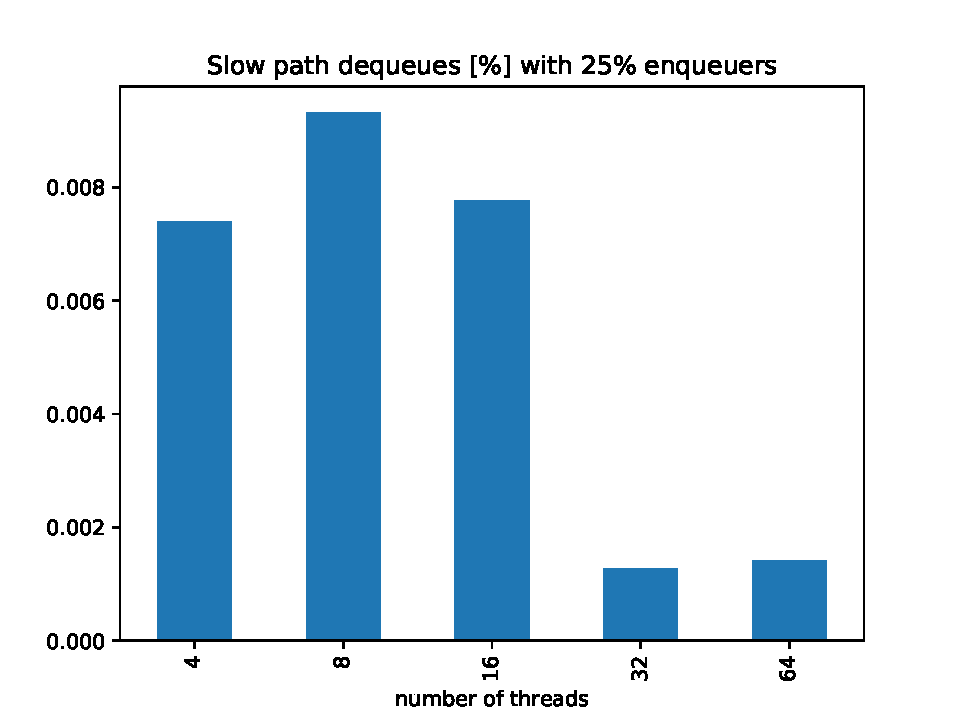
\includegraphics[width=\linewidth]{../benchmark/DEQ_SP_25.pdf}
        \end{minipage}
        \begin{minipage}[b]{0.5\linewidth}
            \centering
            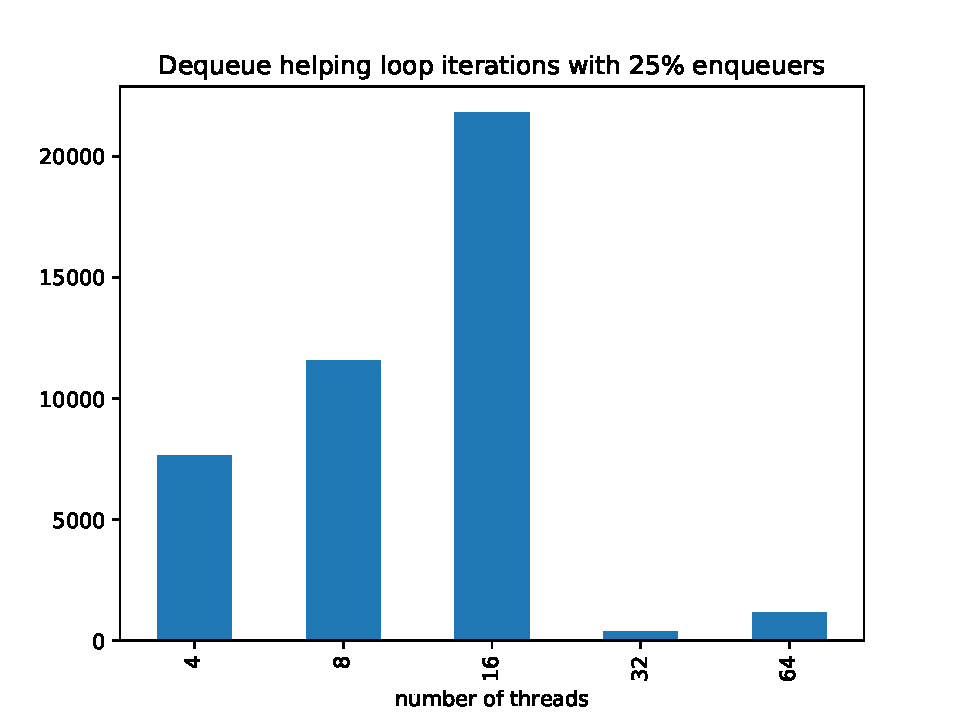
\includegraphics[width=\linewidth]{../benchmark/DEQ_HELP_25.pdf}
        \end{minipage}
    }
    \centerline{
        \begin{minipage}[b]{0.5\linewidth}
            \centering
            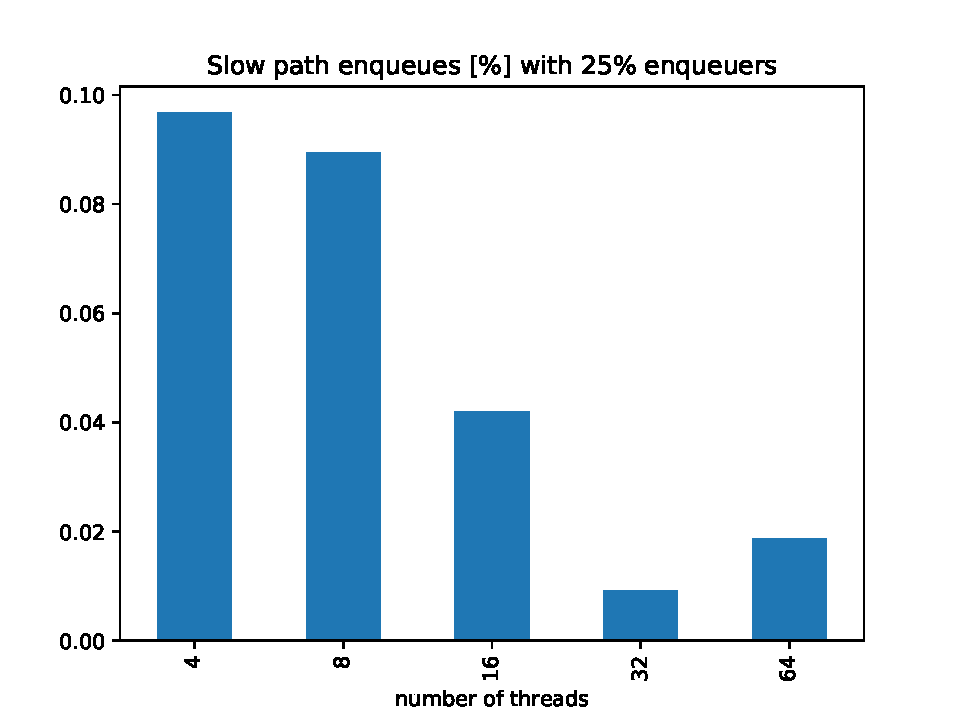
\includegraphics[width=\linewidth]{../benchmark/ENQ_SP_25.pdf}
        \end{minipage}
        \begin{minipage}[b]{0.5\linewidth}
            \centering
            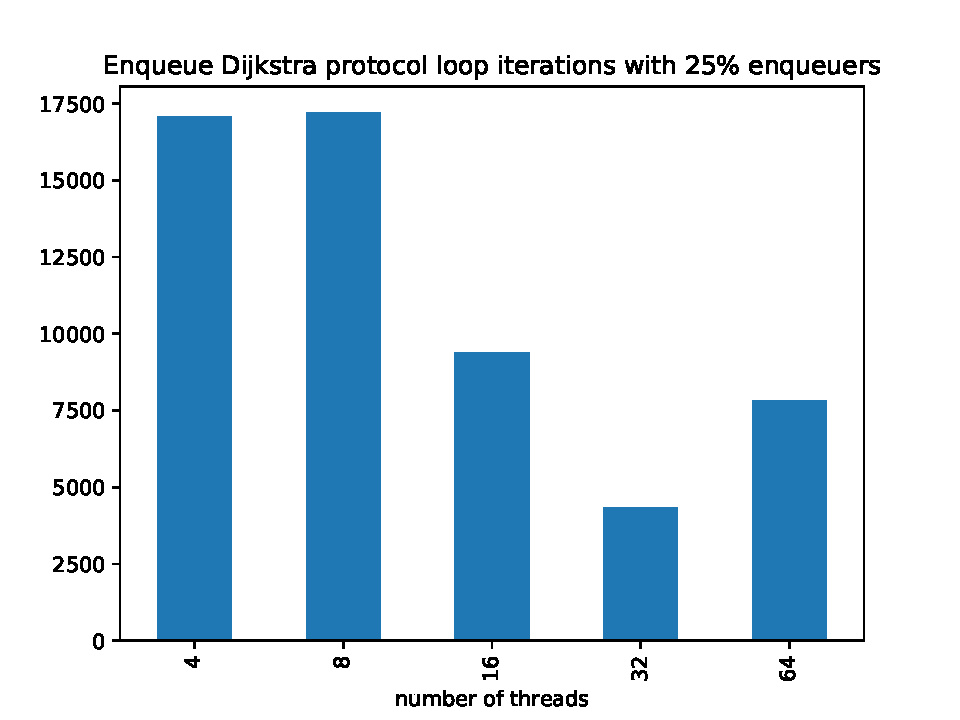
\includegraphics[width=\linewidth]{../benchmark/ENQ_DIJKSTRA_25.pdf}
        \end{minipage}
    }
\end{sidewaysfigure}
\clearpage
\subsection{Conclusion\label{sec:eval-conlusion}}
The conclusion can easily be drawn after all these interpretations about the performance metrics of concurrent queues: linearizability and tight progress guarantees come at a high performance penalty. The \GLQ{} provided a good performance baseline, which was surpassed by the \WFQ{} that is non-blocking and provides a wait-free progress guarantee, which is quite remarkable. On the other hand the \LFQ{} drops linearizability and wait-freedom to increase the data structure throughput and latency to a level, which by far surpasses the \WFQ{}. This can be easily explained by the fact that the \WFQ{} just uses a waiting loop to ensure linearizability, which increases latency and limits the throughput. Maybe the atomic instructions become better in future hardware, but by now atomic operations are very costly if the thread count exceeds about $8$ threads. The overall performance of the various queues is quite nicely shown in the following scatter plots, which include all measured data points:
\clearpage
\begin{sidewaysfigure}
    \centerline{
        \begin{minipage}[b]{0.5\linewidth}
            \centering
            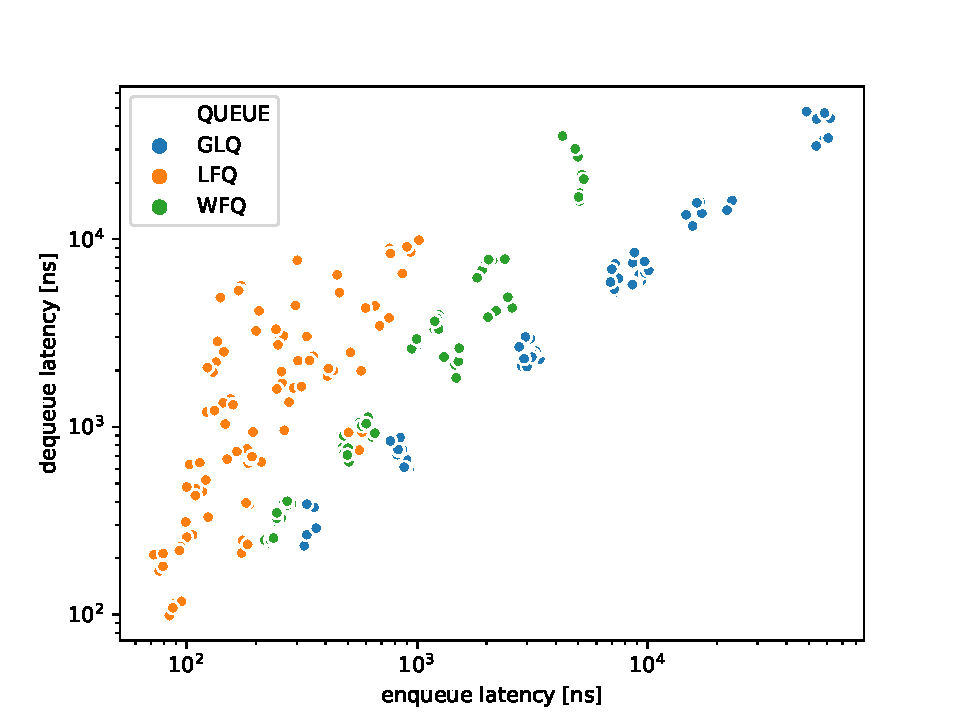
\includegraphics[width=\linewidth]{../benchmark/SCATTER_LAT.pdf}
        \end{minipage}
        \begin{minipage}[b]{0.5\linewidth}
            \centering
            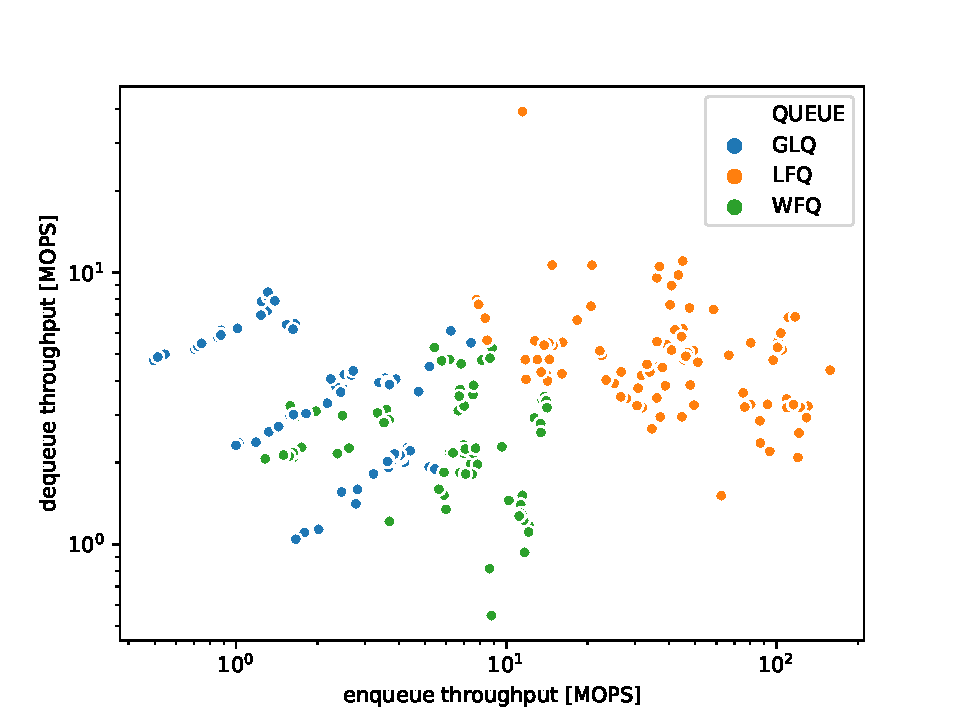
\includegraphics[width=\linewidth]{../benchmark/SCATTER_THROUGH.pdf}
        \end{minipage}
    }
    \centerline{
        \begin{minipage}[b]{0.5\linewidth}
            \centering
            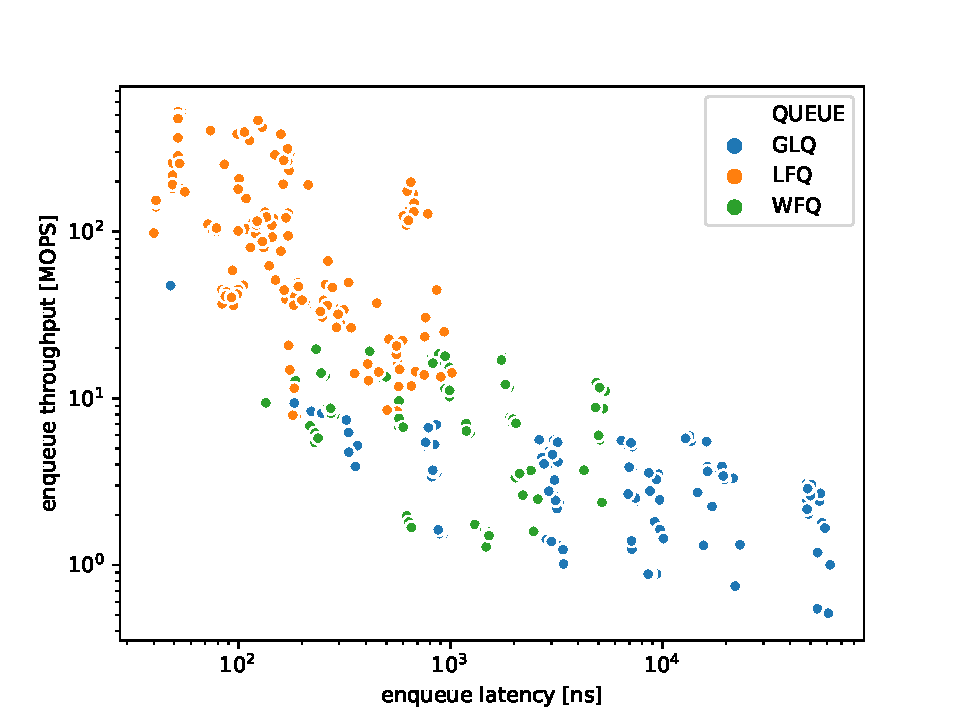
\includegraphics[width=\linewidth]{../benchmark/SCATTER_LAT_THROUGH_ENQ.pdf}
        \end{minipage}
        \begin{minipage}[b]{0.5\linewidth}
            \centering
            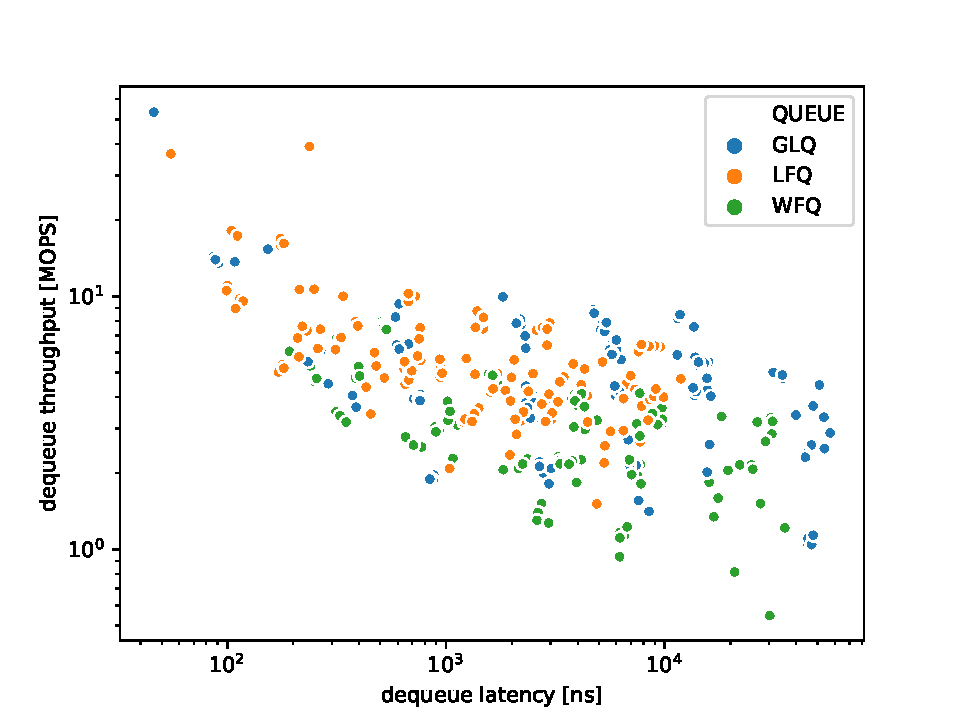
\includegraphics[width=\linewidth]{../benchmark/SCATTER_LAT_THROUGH_DEQ.pdf}
        \end{minipage}
    }
\end{sidewaysfigure}
\clearpage
\begin{sidewaysfigure}
    \subsection{Results\label{sec:eval-results}}
    \subsubsection{Enqueue Throughput\label{sec:eval-results-enq-through}}
    \centerline{
        \begin{minipage}[b]{0.5\linewidth}
            \centering
            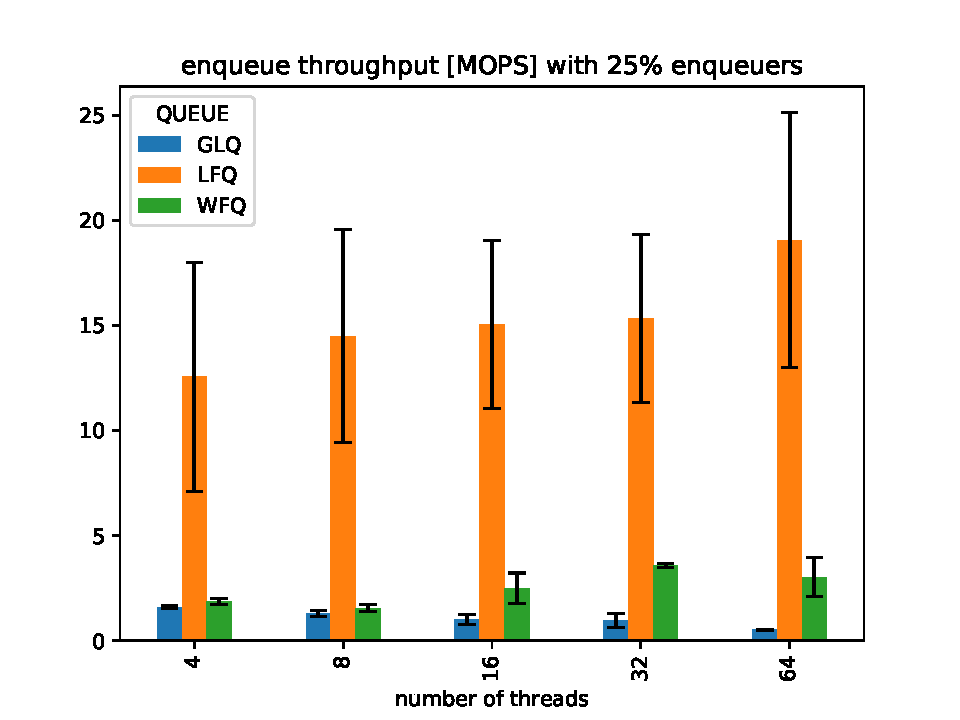
\includegraphics[width=\linewidth]{../benchmark/ENQ_THROUGH_25.pdf}
        \end{minipage}
        \begin{minipage}[b]{0.5\linewidth}
            \centering
            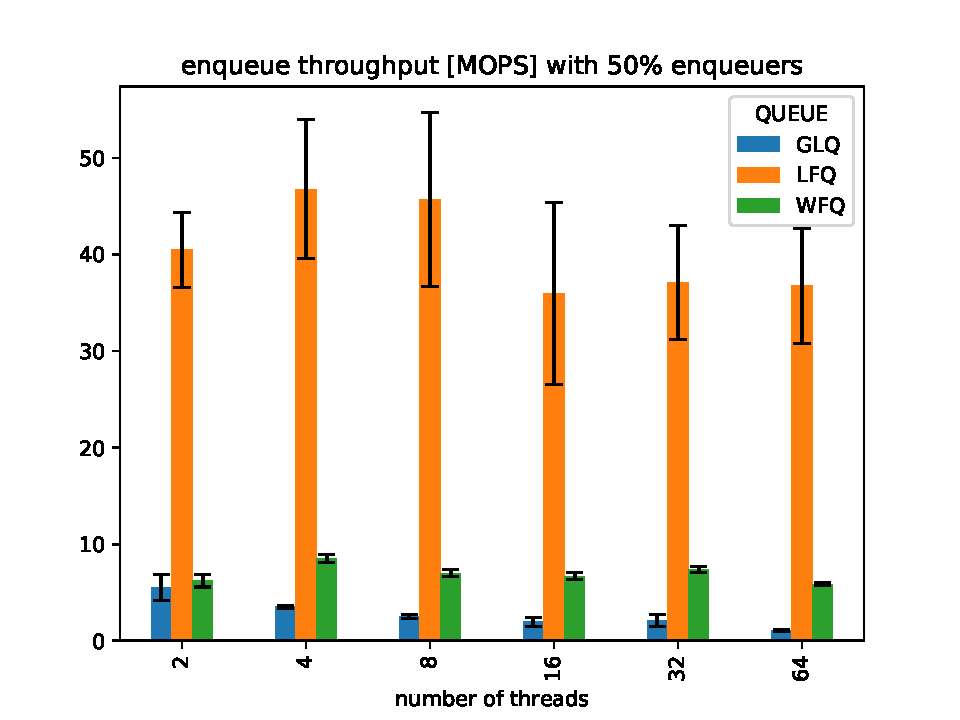
\includegraphics[width=\linewidth]{../benchmark/ENQ_THROUGH_50.pdf}
        \end{minipage}
    }
    \centerline{
        \begin{minipage}[b]{0.5\linewidth}
            \centering
            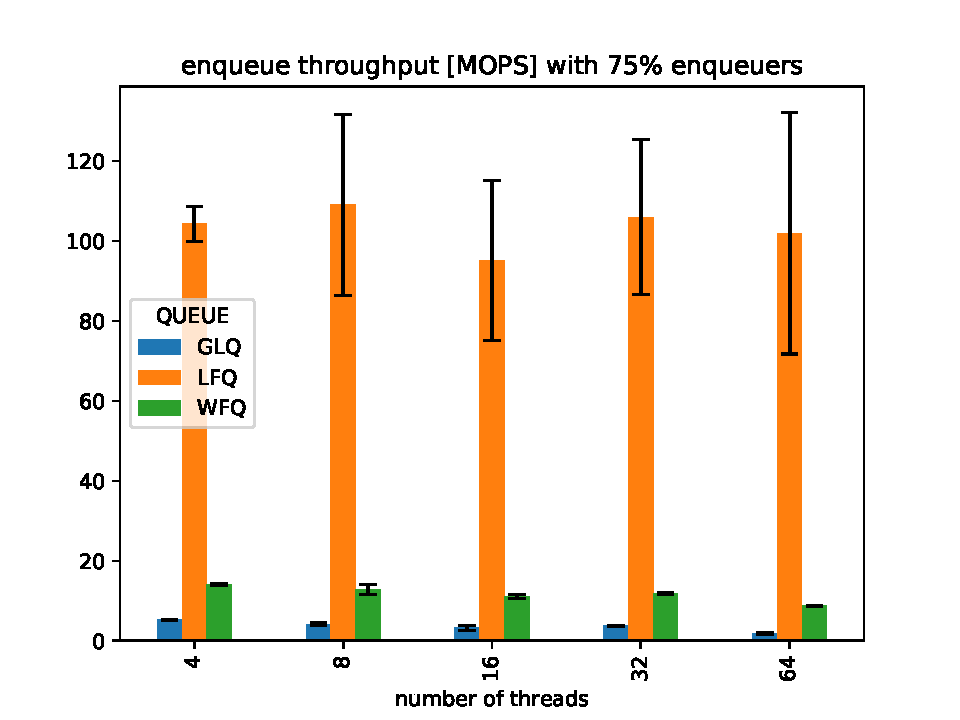
\includegraphics[width=\linewidth]{../benchmark/ENQ_THROUGH_75.pdf}
        \end{minipage}
        \begin{minipage}[b]{0.5\linewidth}
            \centering
            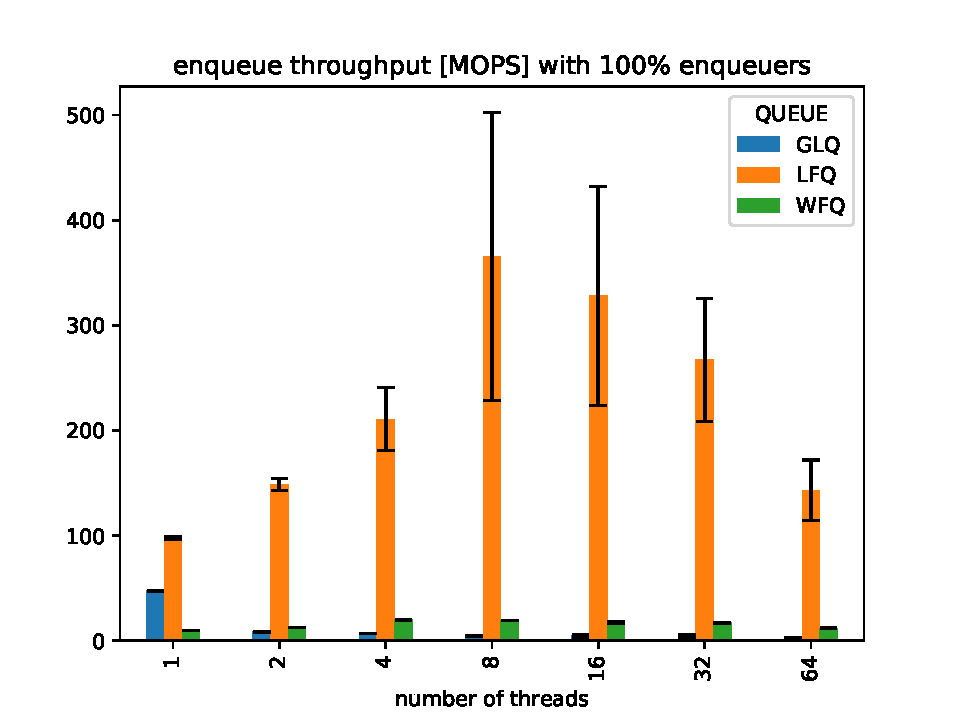
\includegraphics[width=\linewidth]{../benchmark/ENQ_THROUGH_100.pdf}
        \end{minipage}
    }
\end{sidewaysfigure}
\clearpage
    \begin{sidewaysfigure}
        \subsubsection{Deuqueue Throughput\label{sec:eval-results-deq-through}}
        \centerline{
        \begin{minipage}[b]{0.5\linewidth}
            \centering
            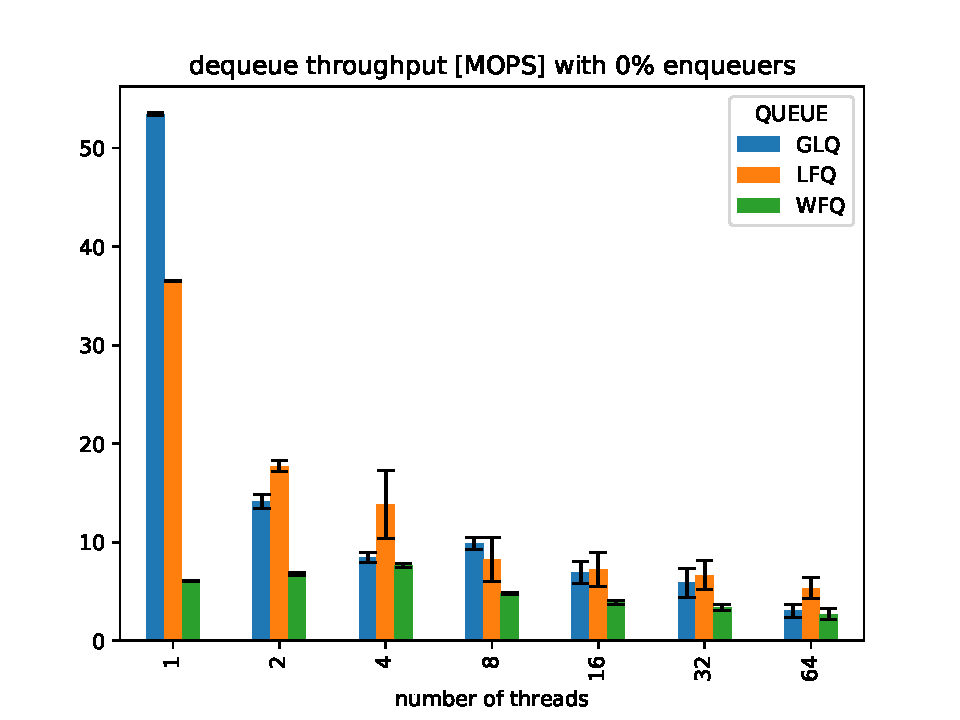
\includegraphics[width=\linewidth]{../benchmark/DEQ_THROUGH_0.pdf}
        \end{minipage}
        \begin{minipage}[b]{0.5\linewidth}
            \centering
            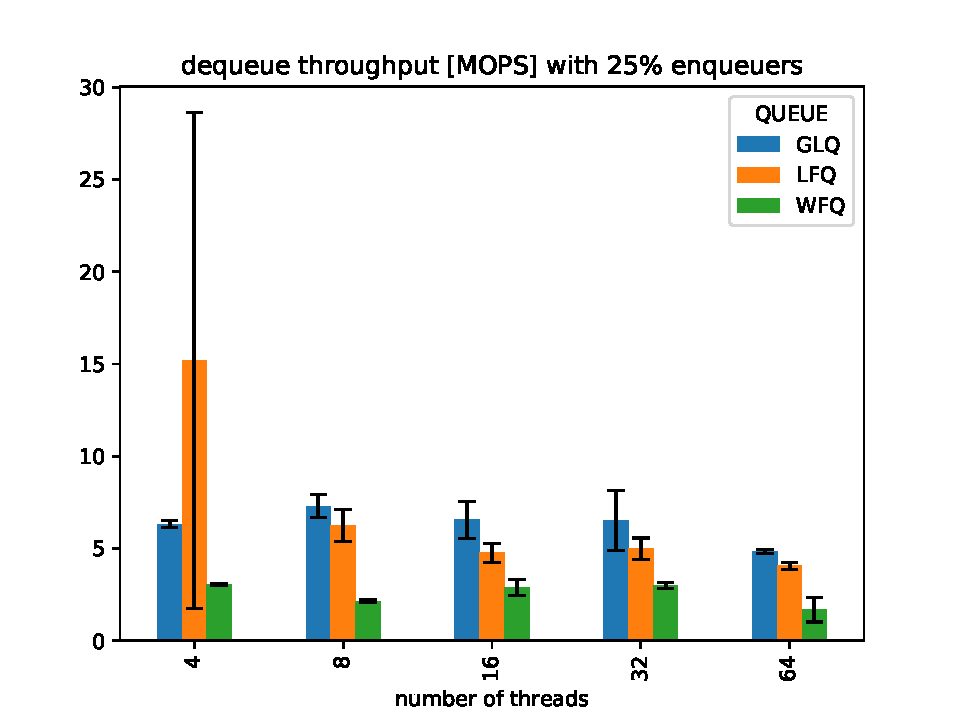
\includegraphics[width=\linewidth]{../benchmark/DEQ_THROUGH_25.pdf}
        \end{minipage}
        }
        \centerline{
        \begin{minipage}[b]{0.5\linewidth}
            \centering
            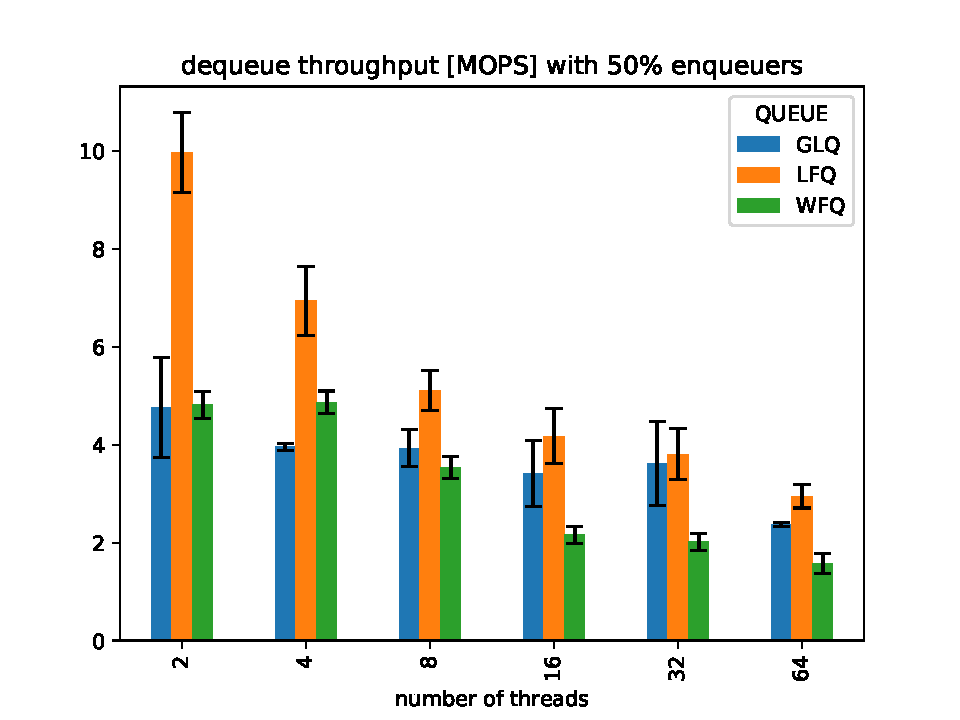
\includegraphics[width=\linewidth]{../benchmark/DEQ_THROUGH_50.pdf}
        \end{minipage}
        \begin{minipage}[b]{0.5\linewidth}
            \centering
            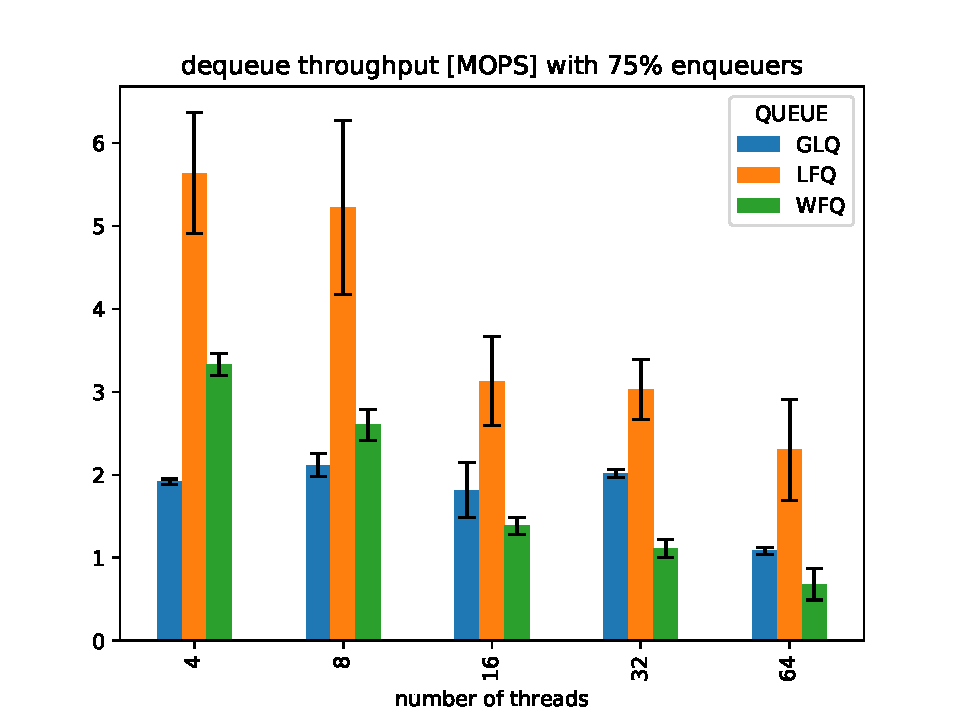
\includegraphics[width=\linewidth]{../benchmark/DEQ_THROUGH_75.pdf}
        \end{minipage}
        }
    \end{sidewaysfigure}
    \clearpage
    \begin{sidewaysfigure}
        \subsubsection{Enqueue Latency\label{sec:eval-results-enq-latency}}
        \centerline{
        \begin{minipage}[b]{0.5\linewidth}
            \centering
            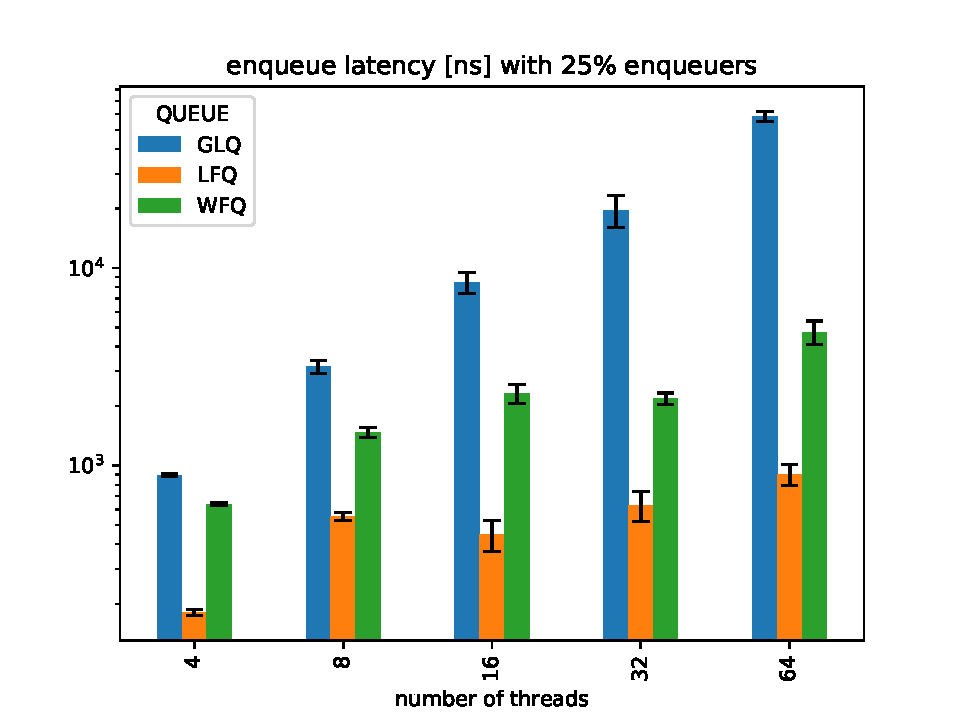
\includegraphics[width=\linewidth]{../benchmark/ENQ_LAT_25.pdf}
        \end{minipage}
        \begin{minipage}[b]{0.5\linewidth}
            \centering
            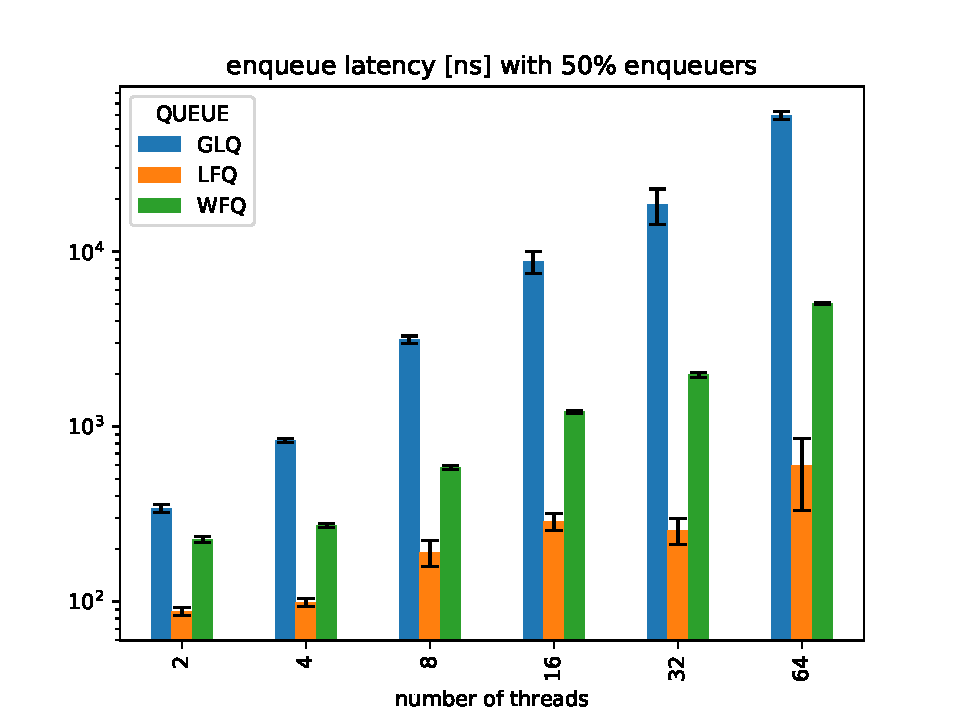
\includegraphics[width=\linewidth]{../benchmark/ENQ_LAT_50.pdf}
        \end{minipage}
        }
        \centerline{
        \begin{minipage}[b]{0.5\linewidth}
            \centering
            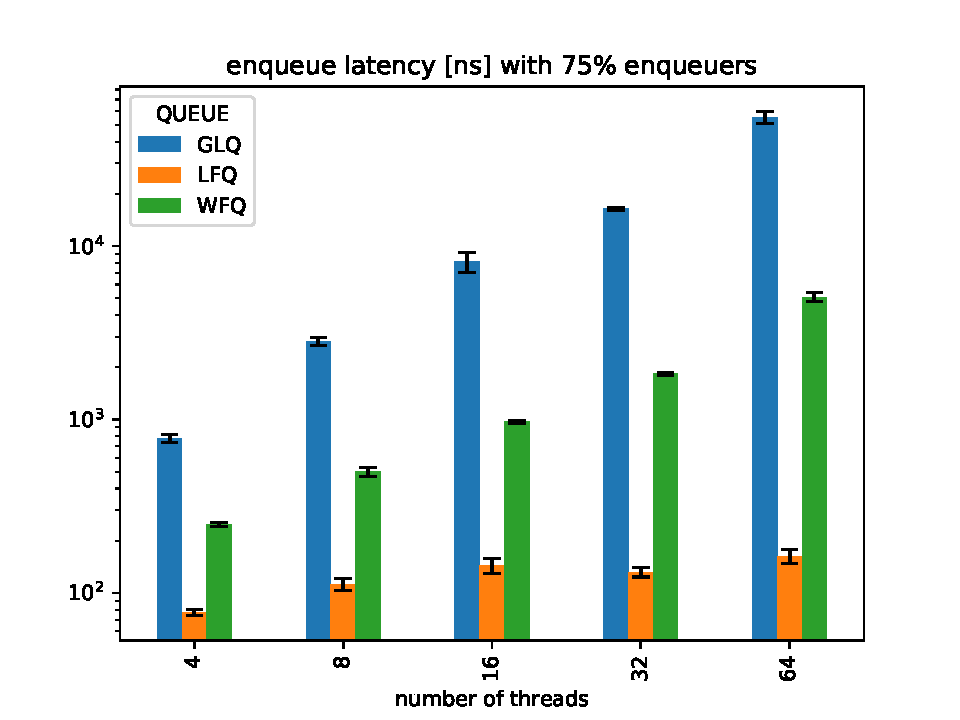
\includegraphics[width=\linewidth]{../benchmark/ENQ_LAT_75.pdf}
        \end{minipage}
        \begin{minipage}[b]{0.5\linewidth}
            \centering
            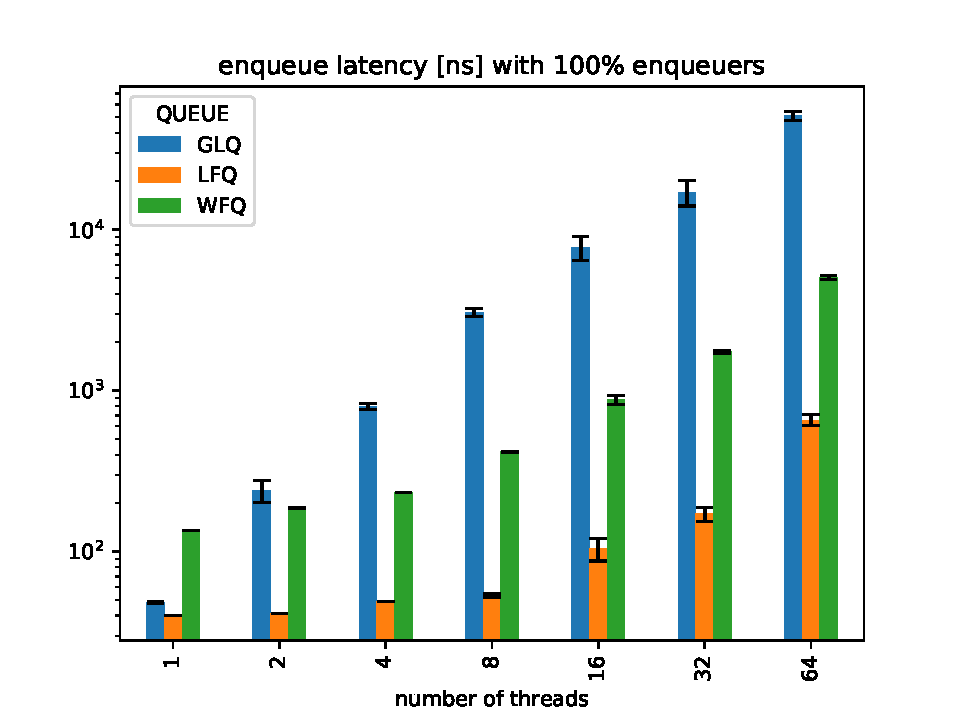
\includegraphics[width=\linewidth]{../benchmark/ENQ_LAT_100.pdf}
        \end{minipage}
        }
    \end{sidewaysfigure}
    \clearpage
    \begin{sidewaysfigure}
        \subsubsection{Deuqueue Latency\label{sec:eval-results-deq-latency}}
        \centerline{
        \begin{minipage}[b]{0.5\linewidth}
            \centering
            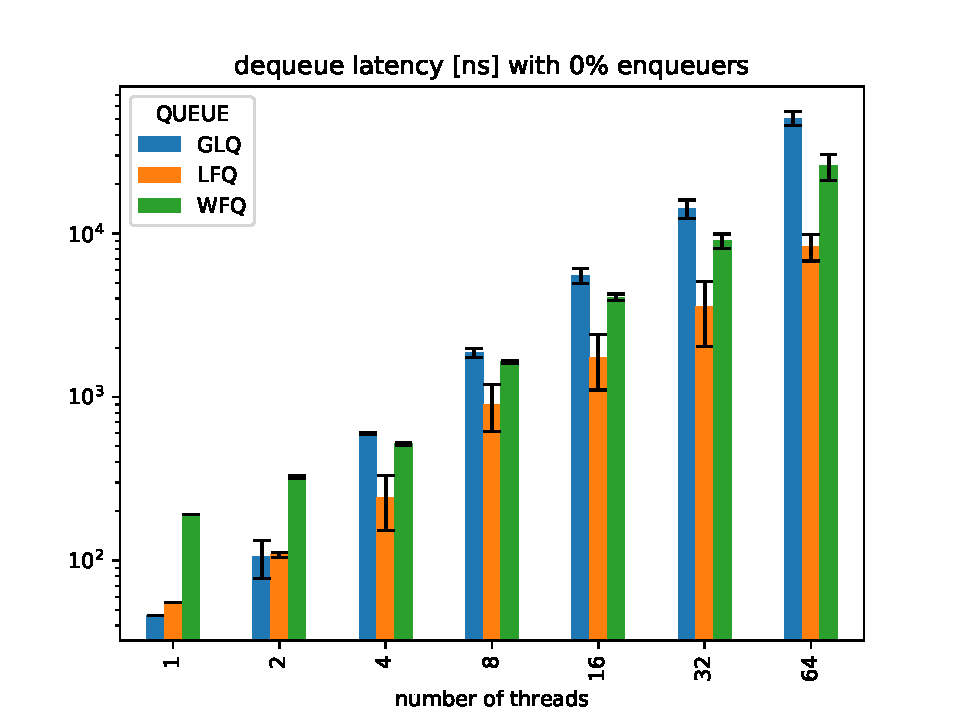
\includegraphics[width=\linewidth]{../benchmark/DEQ_LAT_0.pdf}
        \end{minipage}
        \begin{minipage}[b]{0.5\linewidth}
            \centering
            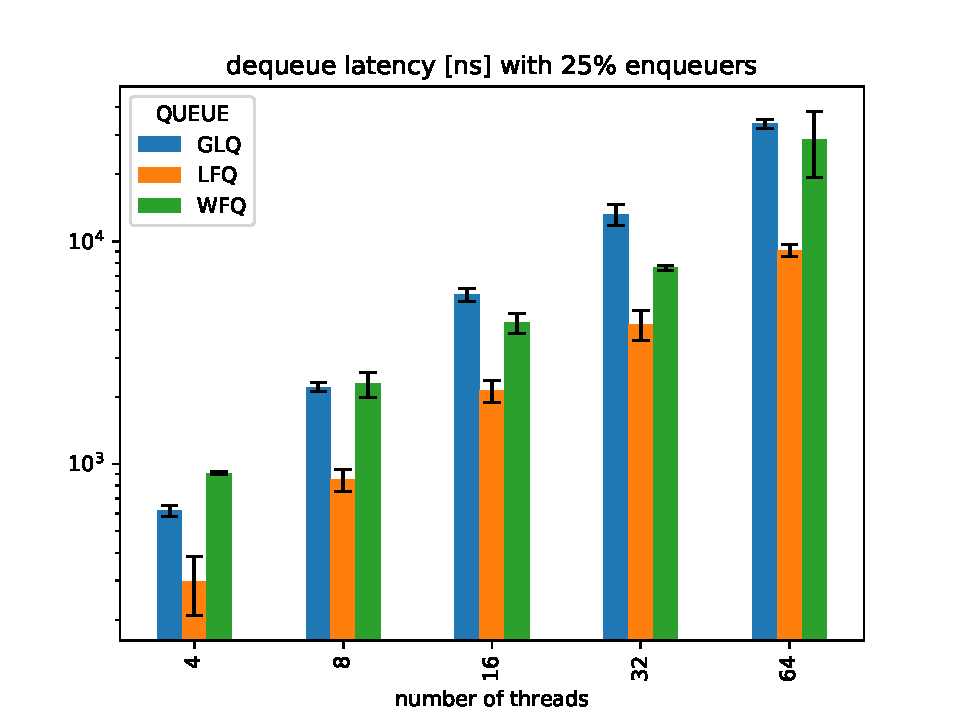
\includegraphics[width=\linewidth]{../benchmark/DEQ_LAT_25.pdf}
        \end{minipage}
        }
        \centerline{
        \begin{minipage}[b]{0.5\linewidth}
            \centering
            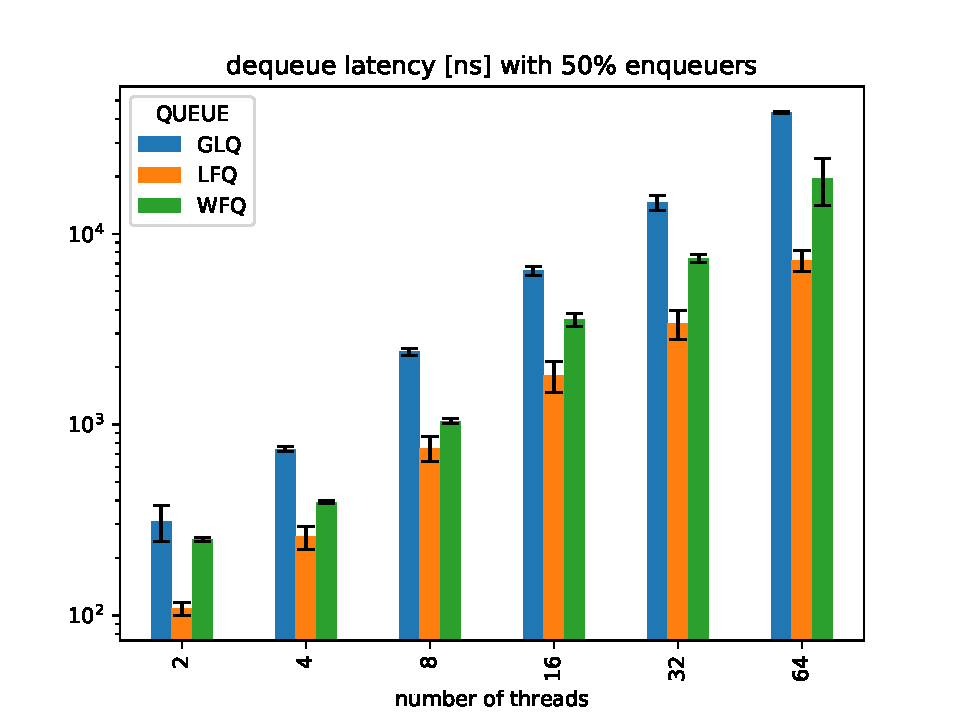
\includegraphics[width=\linewidth]{../benchmark/DEQ_LAT_50.pdf}
        \end{minipage}
        \begin{minipage}[b]{0.5\linewidth}
            \centering
            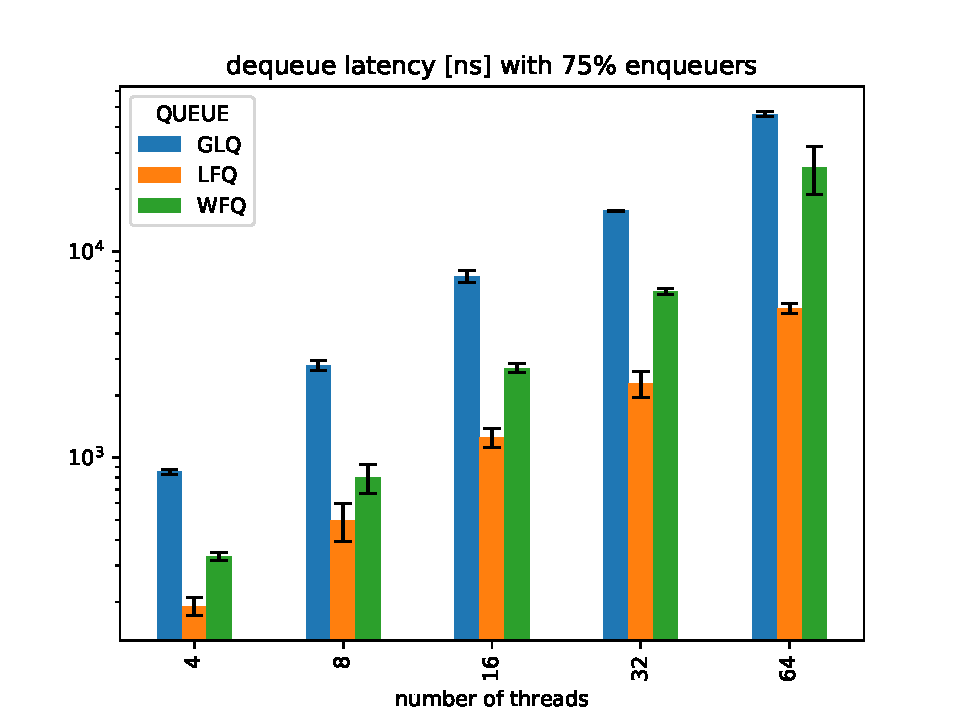
\includegraphics[width=\linewidth]{../benchmark/DEQ_LAT_75.pdf}
        \end{minipage}
        }
    \end{sidewaysfigure}
    \clearpage
    \begin{sidewaysfigure}
    \subsubsection{CAS Failure Percentage \label{sssec:cas}}
    \centerline{
    \begin{minipage}[b]{0.5\linewidth}
        \centering
        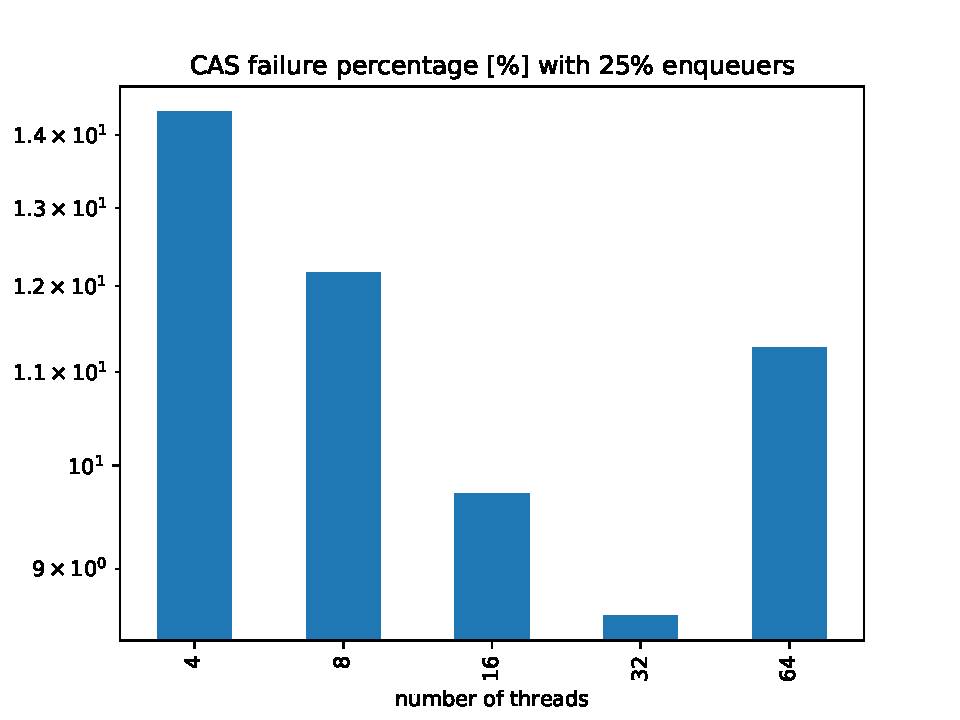
\includegraphics[width=\linewidth]{../benchmark/CAS_CASFAIL_25.pdf}
    \end{minipage}
    \begin{minipage}[b]{0.5\linewidth}
        \centering
        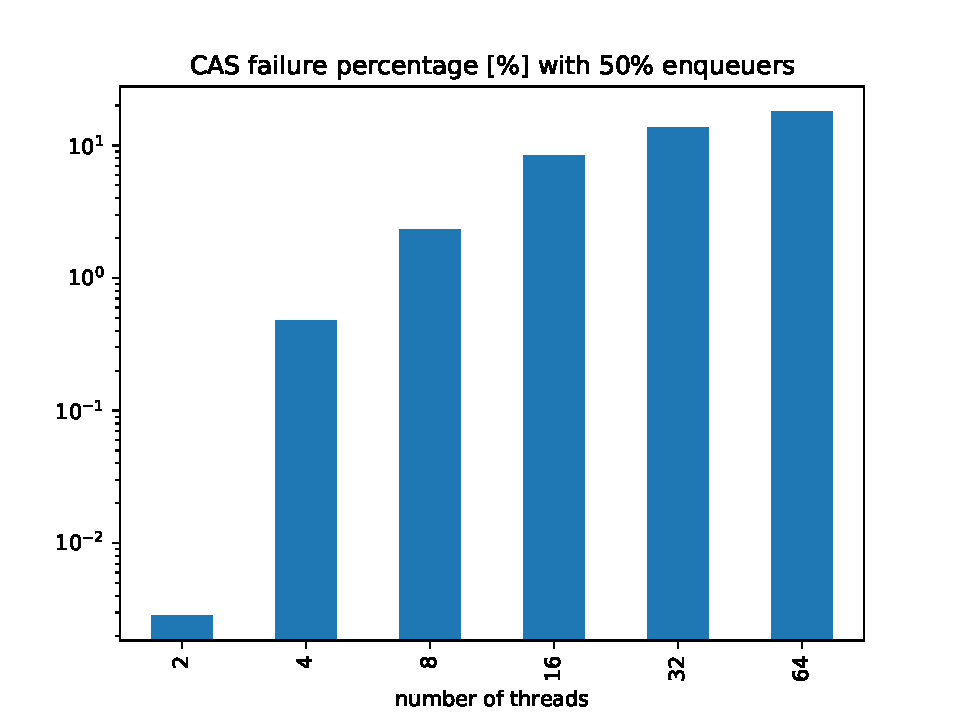
\includegraphics[width=\linewidth]{../benchmark/CAS_CASFAIL_50.pdf}
    \end{minipage}
    }
    \centerline{
    \begin{minipage}[b]{0.5\linewidth}
        \centering
        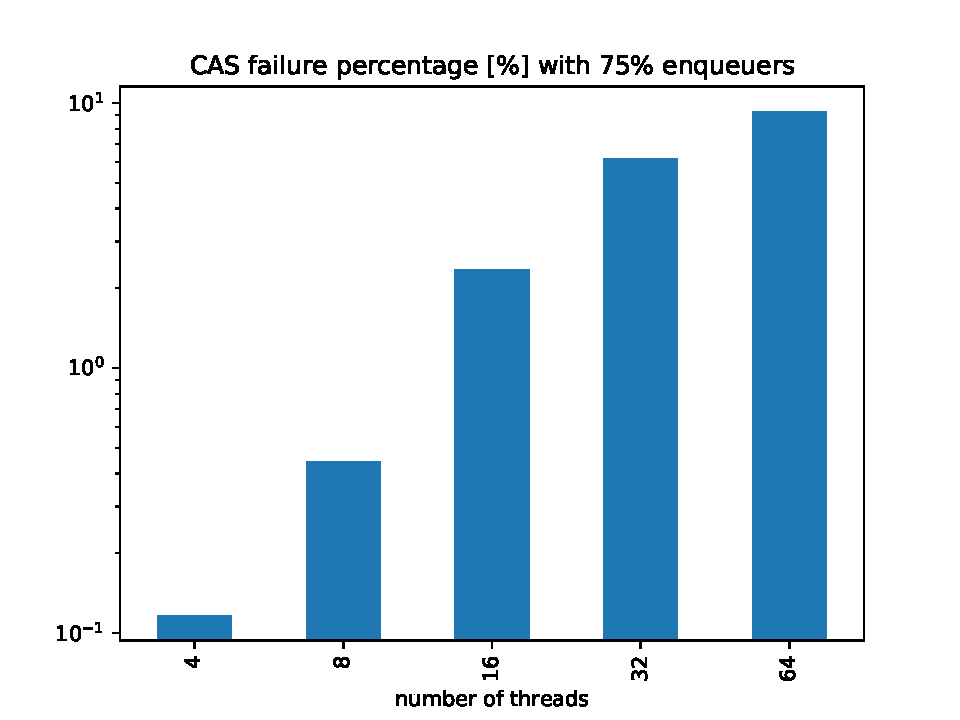
\includegraphics[width=\linewidth]{../benchmark/CAS_CASFAIL_75.pdf}
    \end{minipage}
    \begin{minipage}[b]{0.5\linewidth}
        \centering
        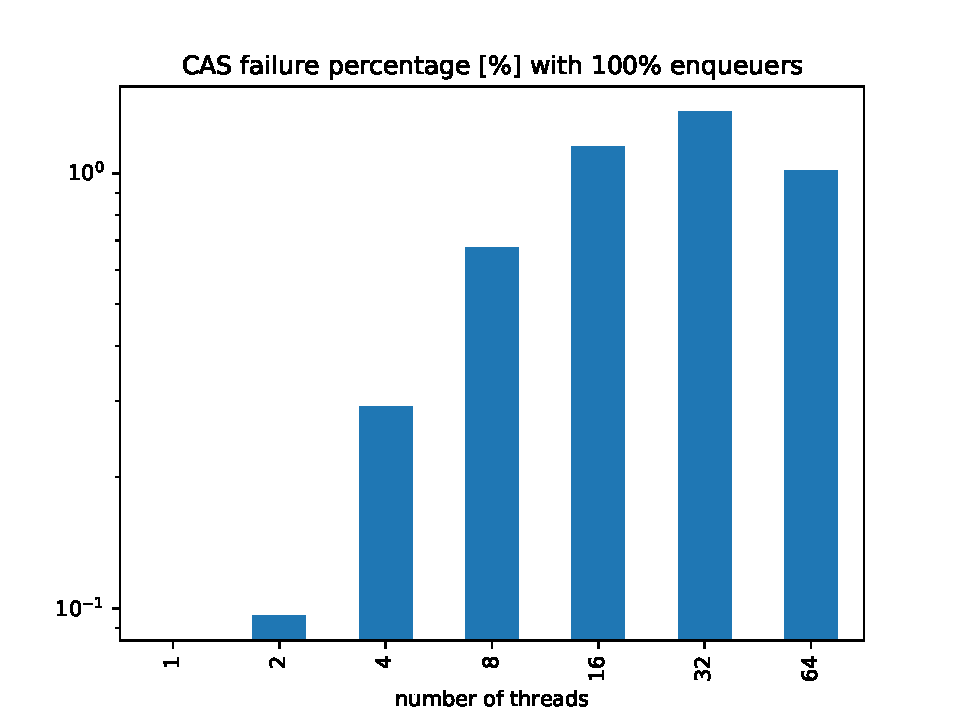
\includegraphics[width=\linewidth]{../benchmark/CAS_CASFAIL_100.pdf}
    \end{minipage}
    }
    \end{sidewaysfigure}
\clearpage
\printbibliography{}
\end{document}